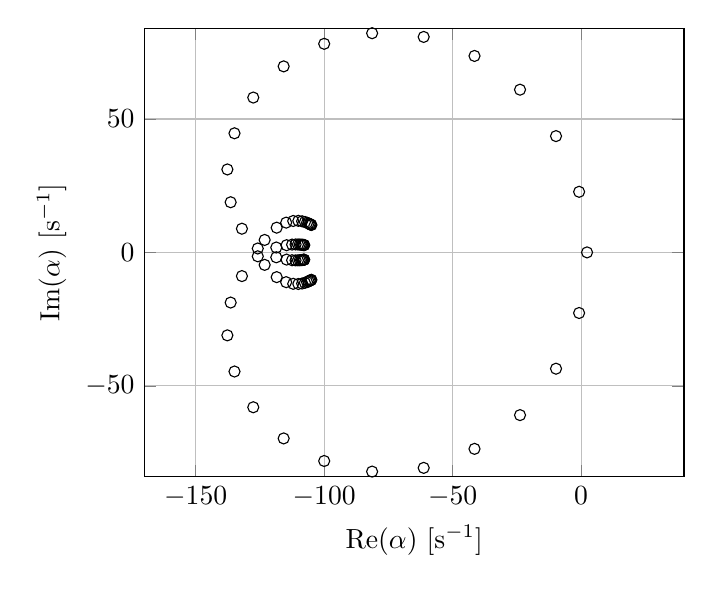
\begin{tikzpicture}
	\begin{axis}[xmin=-170, xmax=40, 
                   ymin=-84, ymax=84, 
                   %extra x ticks={-150,-50,0}, 
                   %extra y ticks={-100,-50,0,50}, 
                   %extra tick style={grid=major}, ]
                   xlabel = {Re($\alpha$) [s$^{-1}$]},
                   ylabel = {Im($\alpha$) [s$^{-1}$]},
                   tick style={grid=major},
                   ]

	\addplot [only marks, mark=o] coordinates {
	(2.291412, 0.000000) 
(-0.801864, 22.705383) 
(-0.801864, -22.705383) 
(-9.783631, 43.575028) 
(-9.783631, -43.575028) 
(-23.793621, 60.968847) 
(-23.793621, -60.968847) 
(-41.507004, 73.614858) 
(-41.507004, -73.614858) 
(-61.283845, 80.738172) 
(-61.283845, -80.738172) 
(-81.352261, 82.131623) 
(-81.352261, -82.131623) 
(-100.003253, 78.160415) 
(-100.003253, -78.160415) 
(-115.774060, 69.701268) 
(-115.774060, -69.701268) 
(-127.598815, 58.024469) 
(-127.598815, -58.024469) 
(-134.909876, 44.633856) 
(-134.909876, -44.633856) 
(-137.680045, 31.084029) 
(-137.680045, -31.084029) 
(-136.403691, 18.795038) 
(-136.403691, -18.795038) 
(-132.020625, 8.876563) 
(-132.020625, -8.876563) 
(-125.852372, 1.461794) 
(-125.852372, -1.461794) 
(-123.173721, 4.669417) 
(-123.173721, -4.669417) 
(-118.491174, 9.268922) 
(-118.491174, -9.268922) 
(-114.800269, 11.150988) 
(-114.800269, -11.150988) 
(-118.641632, 1.835834) 
(-118.641632, -1.835834) 
(-112.063558, 11.769920) 
(-112.063558, -11.769920) 
(-110.061707, 11.831358) 
(-110.061707, -11.831358) 
(-108.590864, 11.656313) 
(-108.590864, -11.656313) 
(-107.501612, 11.395004) 
(-107.501612, -11.395004) 
(-114.640317, 2.695387) 
(-114.640317, -2.695387) 
(-106.690513, 11.119391) 
(-106.690513, -11.119391) 
(-106.086882, 10.864281) 
(-106.086882, -10.864281) 
(-105.642490, 10.646364) 
(-105.642490, -10.646364) 
(-105.324539, 10.473385) 
(-105.324539, -10.473385) 
(-105.111091, 10.348707) 
(-105.111091, -10.348707) 
(-104.988176, 10.273633) 
(-104.988176, -10.273633) 
(-112.492061, 2.931144) 
(-112.492061, -2.931144) 
(-111.140110, 2.982538) 
(-111.140110, -2.982538) 
(-110.210112, 2.970403) 
(-110.210112, -2.970403) 
(-109.534381, 2.935693) 
(-109.534381, -2.935693) 
(-109.027033, 2.894605) 
(-109.027033, -2.894605) 
(-108.639617, 2.854226) 
(-108.639617, -2.854226) 
(-108.342829, 2.817867) 
(-108.342829, -2.817867) 
(-108.118070, 2.787129) 
(-108.118070, -2.787129) 
(-107.774437, 2.734682) 
(-107.774437, -2.734682) 
(-107.953214, 2.762799) 
(-107.953214, -2.762799) 
(-107.840334, 2.745257) 
(-107.840334, -2.745257) 

		};
\end{axis}
\end{tikzpicture}